\chapter{Study 2 - Attentional Networks}
\label{ch:attentional}
To help simplify the learning problem the task was again reframed to improve the signal to noise ratio.
The preprocessing was adjusted such that decay was applied around every event but instead of using the full image only an 11x11 decayed area was kept.
In keeping with previous experiments decay was applied into the past and future to be the input and output. 
Figure \ref{fig:11inoutpair} is an example of such a pair.
%Rather than applying decay to the whole image at uniform time intervals and using that as input the to the network each event was decayed around resulting in many more (albiet similar) training examples.
%However only an 11x11 area around each event was considered meaning the signal to noise ratio was much higher. 

\begin{figure}[h]
    \centering
    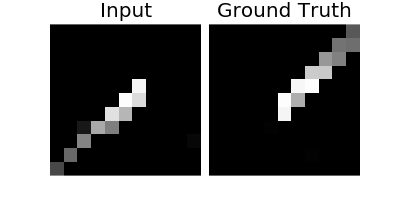
\includegraphics[width=0.8\textwidth]{11xinoutpair_83.png}
    \caption{Example of 11x11 input for an attentional network}
    \label{fig:11inoutpair}
\end{figure}

Figure \ref{fig:11inoutpair} is a cherry picked training example though.
The Attentional networks still have a noisy task to solve because all events, including noise events, are considered. 
Many of the training examples derived from noise pixels could be filtered out efficiently by demmanding the total activity in a training example excede some low threshold.
However, the system should be able to deal with noise and setting such a threshold would create another unnecessary hyper-parameter to the model.
Additonally such a parameter would be dependent on the time scale of the data and would need to be adjusted for each task. 
As will be shown the network is able to learn even in the midst of such noise so it is left in. 

%%%%%%%%%%%%%%%%%%%%%%%%%%%%%%      ATTENTIONAL NN    %%%%%%%%%%%%%%%%%%%%%%%%%%%%%%%%%%%%%%
\section{Attentional Directly Connected (ADC) Network}

\subsection{Aims}
% TODO Need to actually set some aims here
This network, as the name suggests, is a direct connection between the input and output units.
The prediction problem had been broken down into a seemingly simple task so it was expected that results could be achieved with a simple network. 

\subsection{Method}
The network details are outlined in table \ref{tb:attnet1def}, with key points being the loss function has returned to the standard S.S.D. instead of the linearly weighted S.S.D. and the number of inputs has drastically decreased. 

\begin{table}[h]
\centering
\begin{tabular}{ | l | l | }
    \hline
    Num. Inputs & 121 \\
    Num. Outputs & 121 \\
    Connectivity & Fully connected \\
    Num. Hidden Layers & 0 \\
    Activation function & Linear, ReLU, Sigmoid \\
    Loss & Sum of Squares Difference \\
    Learning rule & S.G.D. (back propogation) \\
    Learning rate & 0.1 \\
    Mini-batch size & 100 \\
    \hline
\end{tabular}
\caption{Features of the Attentional Directly Connected Networks}
\label{tb:attnet1def}
\end{table}

\subsection{Linear activation}
The simplest ADC network considered had only a linear activation to compute outputs. 
This proved to be enough for the network to learn to make coherent predictions. 
The two datasets (8 Angle and Arbitrary Angle) were considered, a network was trained on each and then made predictions on a set of validation data from it's own dataset and other dataset to see how it could generalise.
For clarity the network trained on the 8AD will be called 8AngNet and the network trained on the AAD will be called ArbAngNet. 

\subsubsection{Linearly activated 8AngNet results}

\begin{figure}
    \centering
    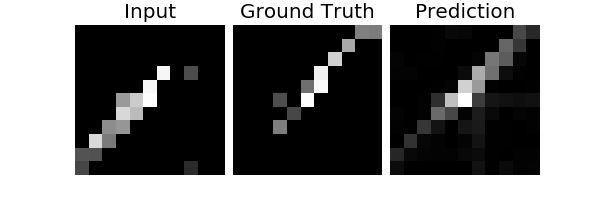
\includegraphics[width=0.8\textwidth]{ADC_8a_8a_13.png}
    \caption{A good prediction from 8AngNet on the 8AD validation set.}
    \label{fig:ADC_8a_8a_crct} 
\end{figure}

\begin{figure}
    \centering
    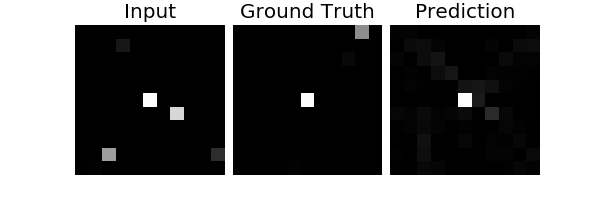
\includegraphics[width=0.8\textwidth]{ADC_8a_8a_7.png}
    \caption{A prediction from 8AngNet with a noisy input}
    \label{fig:ADC_8a_8a_noisy}
\end{figure}

Figures \ref{fig:ADC_8a_8a_crct} and \ref{fig:ADC_8a_8a_noisy} show how the linearly activated 8AngNet predicted in two cases from the 8 Angle validation set.
This prediction looks promising that the network is capable of representing some structure of the data as the prediction is similar to the label (ignoring some noise).
% TODO Make this an even more correct image and use this particular img (13) later to discuss problems
%In figure \ref{fig:ADC_8a_8a_crct} the network is performing well and gives a prediction which is quite similar the ground truth (ignoring noise). 
Figure \ref{fig:ADC_8a_8a_noisy} shows a noisy training example.
The label does not intuitively follow from the input and the network only outputs small values.
However the network does predict faintly along the top left diagonal which is sensible when considering the input has two pixels along the bottom right diagonal (the closer of which is highly active making it resemble a decayed path). 
%However the network has noticed two pixels active along the bottom right diagonal (one of which is highly active) and the network predicts a faint output along the top left diagonal.

\begin{figure}
    \centering
    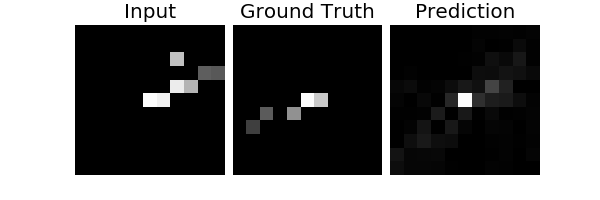
\includegraphics[width=0.8\textwidth]{ADC_8a_aa_4.png}
    \caption{8AngNet struggles to predict inbetween paths}
    \label{fig:ADC_8aNoaa}
\end{figure}

\begin{figure}
    \centering
    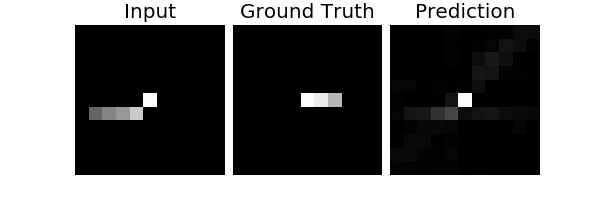
\includegraphics[width=0.8\textwidth]{ADC_8a_aa_46.png}
    \caption{8AngNet predicting a slightly off angle input}
    \label{fig:ADC_8aNoaa_fork}
\end{figure}

The network performing well on its own validation set is a success in itself but raises the question of how it will generalise from 8AD to AAD.
It was hypothesised the network might be able to use a combination of known angles to represent the new angles in the Arbitrary Angle dataset.
This was not the case though, figure \ref{fig:ADC_8aNoaa} shows the network stuggling to predict the motion.
Most of the activity in the prediction falls in the East North-East section which is where the input was.
There is some very limited activity that matches the label but this is insignificant compared to previous predictions and what can be realistically expected from the network. 
Further figure \ref{fig:ADC_8aNoaa_fork} shows a slightly off center input which resembles an angle from 8AD. 
The network has trouble interpreting this and makes 3 very faint predictions being the top right diagonal, to the right edge and along the input.
This suggests the network is not able to efficiently represent the arbitrary angles as some combination of the angles it learnt and could perform reasonably well on.

An additional interesting case which further supports this claim is seen in figure \ref{fig:ADC_8aNoaa_special} which shows the network suffering from some neatly aligned noise. 
The network is well equipped to deal with inputs coming from one angle at a time but this noise makes it appear as if two dots may be crossing paths. 
The networks behaviour to predict two strong output paths shows that each input path (and its predictions) are happening independently of the rest of the input.
If the network was representing the input as an angle it would be reasonable to expect that the output might be a blur in the top right corner of the prediction.  
Instead this clear prediction of two paths suggests the network is simply learning to map between areas of the input to areas of the output. 

\begin{figure}
    \centering
    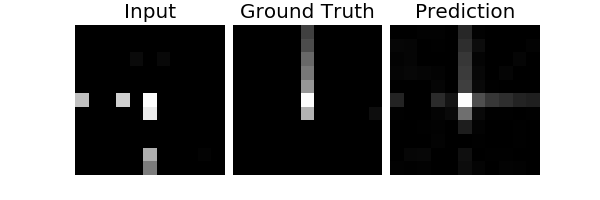
\includegraphics[width=0.8\textwidth]{ADC_8a_aa_15.png}
    \caption{8AngNet network predicting two paths due to noise}
    \label{fig:ADC_8aNoaa_special}
\end{figure}


\subsubsection{Linearly activated ArbAngNet results}
It follows that a network trained on only 8 angles might have trouble generalising to arbitrary angles so a second network was trained on the Arbitrary Angles Dataset. 
In general the network trained on Arbitrary Angle data was less confident in its predictions (magnitude of predictions were lower) but in each guess it would cover a boarder area. 
% TODO rewrite this sentence
An example of this is figure \ref{fig:ADC_aaaa_crct} in which the prediction has many faintly coloured squares, in contrast to the more confident predictions made in figure \ref{fig:ADC_8a_8a_crct} by 8AngNet.

\begin{figure}[h]
    \centering
    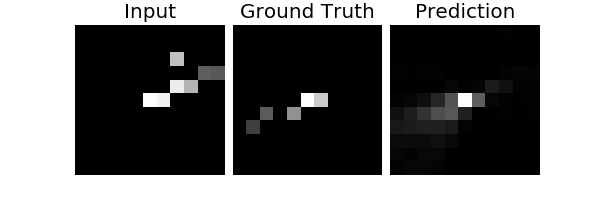
\includegraphics[width=0.8\textwidth]{ADC_aa_aa_4.png}
    \caption{ArbAngNet correctly predicting}
    \label{fig:ADC_aaaa_crct}
\end{figure}
% TODO these visualisations can be improved by grouping the predictions from both nets into 1 img


\begin{figure}[h]
    \centering
    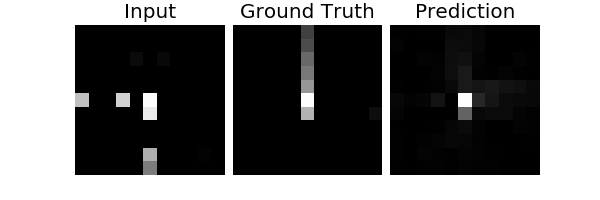
\includegraphics[width=0.8\textwidth]{ADC_aa_aa_15.png}
    \caption{ArbAngNet predicting two paths due to noise}
    \label{fig:ADC_aaaa_twopath}
\end{figure}

\begin{figure}[h]
    \centering
    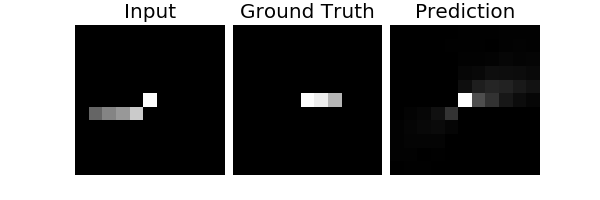
\includegraphics[width=0.8\textwidth]{ADC_aa_aa_46.png}
    \caption{ArbAngNet predicting a slightly off angle input}
    \label{fig:ADC_aaaa_fork}
\end{figure}


The neat noise example which suggested that 8AngNet was simply mapping regions in the input to regions in the output shows a very different prediction from ArbAngNet.
ArbAngNet does not predict any given angle strongly but instead has a very faint prediction along both but also between the two lines. 
The significance of these prediction is questionable given small the predictions are but it does give some insight into the networks dynamics.
It should be noticed that this does not exclude the possibility that ArbAngNet is also just mapping between regions of the input and output, rather this is still a promising theory.

\subsection{Non-linear acitivation}
Compare Sigmoidal with relu?

\subsubsection{Sigmoid activation}
Talk about both 8AD and AAD here

\subsubsection{ReLU activiation}
Talk about both 8AD and AAD here 

\subsection{Attentional Directly Connected network discussion}
How did they go generally?

%%%%%%%%%%%%%%%%%%%%%%%%%%%%%%      ATTENTIONAL NN    %%%%%%%%%%%%%%%%%%%%%%%%%%%%%%%%%%%%%%
\section{Attentional Hidden Layer (AHL) Network}

\subsection{Aims}
 using a hidden layer, what can learn? maybe line params, 1, 2, more hiddens

\subsection{Method}

\subsection{Results}
\subsubsection{1 hidden unit}

\subsubsection{2 hidden units}

\subsubsection{Many hidden units}

\subsection{Discussion}


%%%%%%%%%%%%%%%%%%%%%%%%%%%%%%      AUTO ENCODE     %%%%%%%%%%%%%%%%%%%%%%%%%%%%%%%%%%%%%%
\section{Auto Encoder}
How much could be cleaned up \\
Retry other networks with cleaned up data -- How do they go? \\

